\subsection{Entity-Relationship Schema}

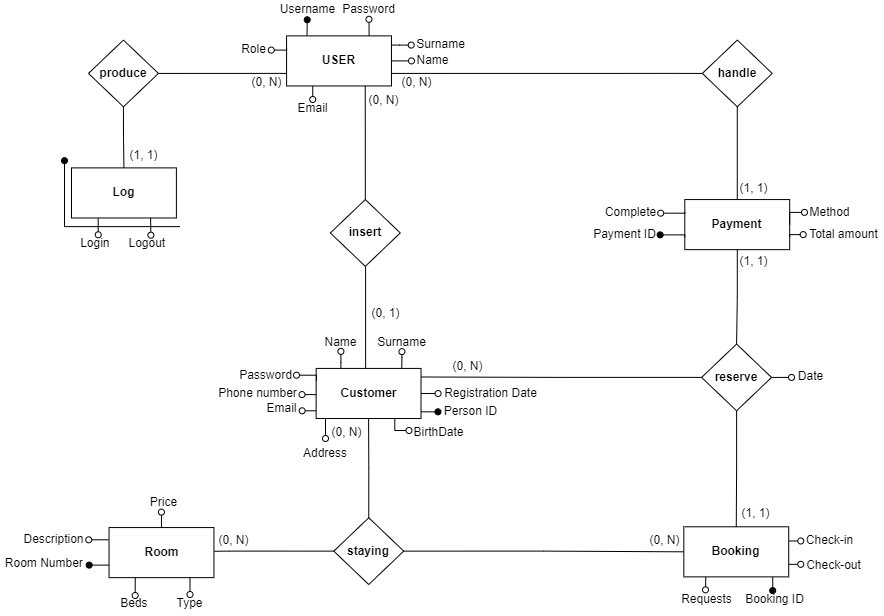
\includegraphics[width=\columnwidth]{images/hotel_ERschema.png}

\noindent The entity-relationship contains 6 main entities:
\begin{itemize}
    \item User: contains the basic information about the users. Each user has, as primary key, their Username(CHAR). For each user we also record Surname(CHAR), Name(CHAR), email(CHAR), Role(ENUM) and password(CHAR). Note that the password is hashed through md5 before storing it.
    \item Customer: the main entity of the database. Contains other additional information about the user. Person ID is a primary key. Phone number (CHAR), Address(CHAR), Registration Data(DATE), BirthDate(DATE).
    \item Log:  made by users. The Log entity represents data for logging purposes. The entity Log keeps the data of the login and the logout of each user accessing the database through the produce relationship.
    \item Payment: Payment ID (ENUM) is a primary key which identificat the number of the payment. For each payment we also know the Method(ENUM): Visa, MasterCard, Maestro, American Express, PayPal, Cash; Total amount(CHAR); Complete(BOOL).
    \item Booking: each has an ID as primary key, is associated with : the personID of the customer who made it; the checkin and checkout timestamps of the staying; the paymentID created as soon as the booking is made; the date in which the booking has been made; optional text type requests.
    \item Room: each is identified by its unique Room Number, which is of type text since it can contain also characters. 
    In the entity are present also the attributes : number of beds, its price, the room type which is of category type plus a description of this type. 
\end{itemize}